% !TEX TS-program = pdflatex
% !TEX encoding = UTF-8 Unicode


\documentclass[12pt]{article} 

\usepackage[utf8]{inputenc} % set input encoding. utf8 or greater 4 lyfe. 

%%% PAGE DIMENSIONS
\usepackage{geometry} % to change the page dimensions
\geometry{a4paper} 
%\geometry{margin=2in} % for example, change the margins to 2 inches all round
% \geometry{landscape} % set up the page for landscape
%   read geometry.pdf for detailed page layout information

\usepackage{graphicx} % support the \includegraphics command and options

% \usepackage[parfill]{parskip} % Activate to begin paragraphs with an empty line rather than an indent

%%% PACKAGES
\usepackage{booktabs} % for much better looking tables
\usepackage{array} % for better arrays (eg matrices) in maths
\usepackage{paralist} % very flexible & customisable lists (eg. enumerate/itemize, etc.)
\usepackage{verbatim} % adds environment for commenting out blocks of text & for better verbatim
\usepackage{subfig} % make it possible to include more than one captioned figure/table in a single float
% These packages are all incorporated in the memoir class to one degree or another...
\usepackage{listings} % for code segment environments.
% see http://en.wikibooks.org/wiki/LaTeX/Source_Code_Listings
\usepackage{tikz} % for FSM drawings from http://madebyevan.com/fsm/
\usepackage{float} % unlocks [H] for float-placement.

%%% HEADERS & FOOTERS
\usepackage{fancyhdr} % This should be set AFTER setting up the page geometry
\pagestyle{fancy} % options: empty , plain , fancy
\renewcommand{\headrulewidth}{0pt} % customise the layout...
% headers
\lhead{TDT4205 Compiler Design, spring 2014}\chead{}\rhead{[trondrud]}
% footers
\lfoot{}\cfoot{\thepage}\rfoot{}

%%% SECTION TITLE APPEARANCE
\usepackage{sectsty}
% \allsectionsfont{\sffamily\mdseries\upshape} % (See the fntguide.pdf for font help)
% (This matches ConTeXt defaults)
\setcounter{secnumdepth}{0}

%%% ToC (table of contents) APPEARANCE
\usepackage[nottoc,notlof,notlot]{tocbibind} % Put the bibliography in the ToC
\usepackage[titles,subfigure]{tocloft} % Alter the style of the Table of Contents
\renewcommand{\cftsecfont}{\rmfamily\mdseries\upshape}
\renewcommand{\cftsecpagefont}{\rmfamily\mdseries\upshape} % No bold!


\title{TDT4205 Compiler Design\\
Assignment 02\\
\textbf{Lexical analysis and parsing}}
\author{Odd M. Trondrud}
%\date{} % Activate to display a given date or no date (if empty),
         % otherwise the current date is printed 

\begin{document}
\maketitle

% you should put the words in here
\part{Theory}
\section{Problem 1, Regular languages}
\subsection{a) Convert the regular expression \texttt{a(b|c)d*e} to a NFA.}
Well, okay, figure~\ref{fig:1-1-a} is a DFA but hey, a DFA is technically a NFA so it's fine. \textit{Sshhh}.
\begin{figure}[H]
\begin{center}
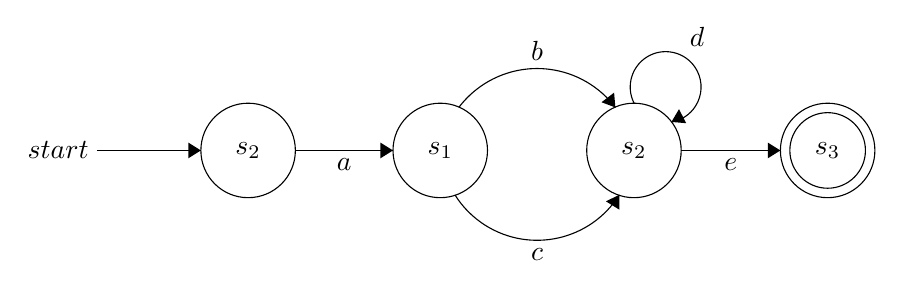
\begin{tikzpicture}[scale=0.2]
\tikzstyle{every node}+=[inner sep=0pt]
\draw [black] (19.7,-31.8) circle (3);
\draw (19.7,-31.8) node {$s_2$};
\draw [black] (31.9,-31.8) circle (3);
\draw (31.9,-31.8) node {$s_1$};
\draw [black] (44.2,-31.8) circle (3);
\draw (44.2,-31.8) node {$s_2$};
\draw [black] (56.5,-31.8) circle (3);
\draw (56.5,-31.8) node {$s_3$};
\draw [black] (56.5,-31.8) circle (2.4);
\draw [black] (10.1,-31.8) -- (16.7,-31.8);
\draw (9.6,-31.8) node [left] {$start$};
\fill [black] (16.7,-31.8) -- (15.9,-31.3) -- (15.9,-32.3);
\draw [black] (22.7,-31.8) -- (28.9,-31.8);
\fill [black] (28.9,-31.8) -- (28.1,-31.3) -- (28.1,-32.3);
\draw (25.8,-32.3) node [below] {$a$};
\draw [black] (33.077,-29.072) arc (142.88868:37.11132:6.236);
\fill [black] (43.02,-29.07) -- (42.94,-28.13) -- (42.14,-28.74);
\draw (38.05,-26.1) node [above] {$b$};
\draw [black] (43.271,-34.621) arc (-32.16924:-147.83076:6.167);
\fill [black] (43.27,-34.62) -- (42.42,-35.03) -- (43.27,-35.56);
\draw (38.05,-38.01) node [below] {$c$};
\draw [black] (44.216,-28.812) arc (207.43495:-80.56505:2.25);
\draw (48.21,-25.26) node [above] {$d$};
\fill [black] (46.58,-29.99) -- (47.52,-30.07) -- (47.06,-29.18);
\draw [black] (47.2,-31.8) -- (53.5,-31.8);
\fill [black] (53.5,-31.8) -- (52.7,-31.3) -- (52.7,-32.3);
\draw (50.35,-32.3) node [below] {$e$};
\end{tikzpicture}

\caption{NFA for the regular expression \texttt{a(b|c)d*e}.}
\label{fig:1-1-a}
\end{center}
\end{figure}



\end{document}
